\chapter{Ist-Analyse}
\label{ch:Ist-Analyse}


	
	\section{Technischer Aufbau}
	\label{ch:ist-aufbau}
	23 Gesellschaften der \ac{ABB} AG machen von der \ac{LLE} für ihre Lieferungen Gebrauch. Viele von diesen Gesellschaften haben eine eigene Variante des Formulars. Die Dokumente unterscheiden sich meistens durch die Position des Briefkopfes oder im Firmenlogo. 
	
	Aktuell wird das Formular mit "`Smart Forms"' umgesetzt. Smart Forms ist eine Formular-Technologie, entwickelt von SAP SE, welche seit Ende 1999 verfügbar ist. Damals sollte diese Variante der Dokumenterstellung den Bedarf an Programmierern für solche Formulare verringern. Mit Hilfe eines \ac{GUI} und anderen Werkzeugen sollte das Erstellen und Verwenden von Dokumenten im SAP ohne eigene Programmierung ermöglicht werden.\footnote{Vgl. \cite{Hertleif.2003} S. 13}  
	
	In der Abbildung \ref{AufLLE} ist der inhaltliche Aufbau der \ac{LLE} dargestellt. 
	\begin{figure}[ht]
		\centering
		\makebox[\textwidth][c]{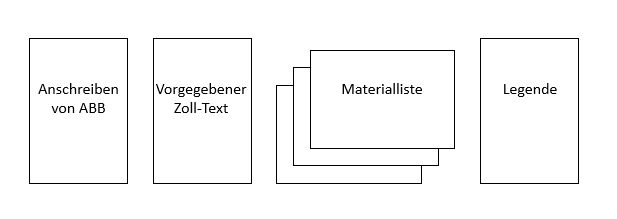
\includegraphics[width=1\textwidth]{img/LLE.png}}%		
		\caption{Aufbau der Lieferantenerklärung}
		\label{AufLLE}
		
	\end{figure}
	
	Das zweiseitige Anschreiben, der Zoll-Text und die Legende werden im Hochformat, die Materialliste wiederum im Querformat ausgegeben. Die Liste kann beliebig lang sein und wird auf neue Seiten mit demselben Layout umgebrochen. Alle Varianten der \ac{LLE} sind zu einem Formular zusammengetragen. Die variablen Inhalte, welche sich von Gesellschaft zu Gesellschaft unterscheiden, werden mit Hilfe von Anzeigebedingungen gesteuert. Die meisten Unterschiede befinden sich auf dem Anschreiben des Dokuments. Unterschiedliche Logos sowie verschiedene Positionen und Ausprägungen der Adressfelder sorgen für eine unübersichtliche Vorschau im "`Form Painter"' in Smart Forms. Der Form Painter zeigt eine Vorschau des Dokumenten-Layouts, ohne dabei die Inhalte der verschiedenen Felder zu berücksichtigen.\footnote{Vgl. \cite{Hertleif.2003} S. 79-81}
	In Abbildung \ref{fig2} ist zu sehen, wie unübersichtlich dieses Layout im Fall der \ac{LLE} aussieht. Sobald Änderungen am Inhalt des Dokumentes vonnöten sind, müssen demnach alle Varianten des Formulars beachtet werden, um Fehler zu vermeiden. Dies führt zu erhöhtem Pflegeaufwand, sowie einem verlängertem Anpassungsprozess.
	
	\begin{figure}[ht]
		\centering
		\makebox[\textwidth][c]{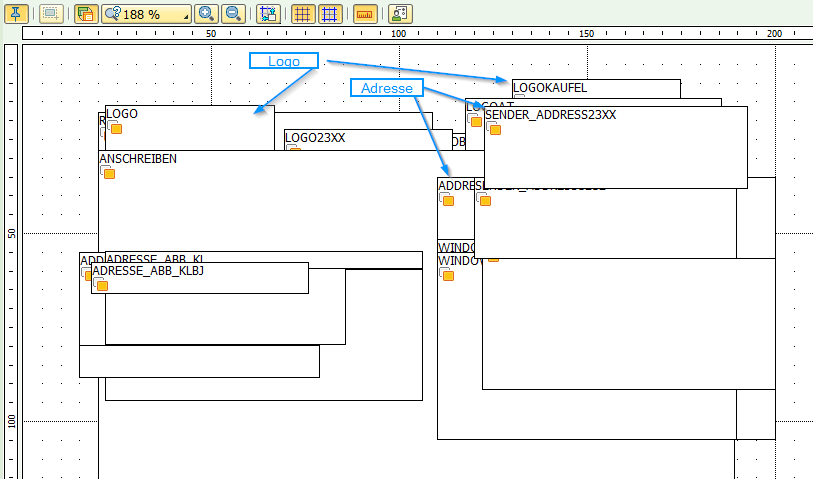
\includegraphics[width=1\textwidth]{img/Smartform-Beispiel-1.png}}%		
		\caption{Lieferantenerklärung in Smart Forms}
		\label{fig2}
	\end{figure}
	
	Ein Ergebnis beim Zusammenführen der verschiedenen Varianten des Formulars in Smart Forms ist auch, dass die verwendeten Texte an unterschiedlichen Stellen hinterlegt sind. Für den einen Teil der Texte werden Textbausteine verwendet, welche unabhängig von Formularen geändert werden können. Diese Bausteine werden im Formular aufgerufen. Der andere Teil der Texte ist jedoch direkt im Smart Form als Textfeld mit festem Inhalt angelegt. 
	
	Diese Inkonsistenz wird weiter in Form von kleinen \ac{ABAP}-Code-Abschnitten in dem Formular geführt, welche die Formulardaten weiterverarbeiten sollen. Diese kleineren Funktionen sind auf dem ganzen Formular verteilt. Oftmals ist nicht erkennbar, wofür ein kleiner Codeabschnitt zuständig ist.
	
	Diese Punkte sorgen dafür, dass der Änderungsprozess zusätzlich verlängert wird. Bei einem so komplexen Dokument muss grundsätzlich mehr Zeit eingeplant werden, da oftmals Mitarbeiter an dem Dokument Änderungen vornehmen müssen, ohne sich vorher mit dem Formular befasst zu haben.\footnote{Durch den Einsatz von externen Dienstleistern ist dies oft der Fall} Der Einarbeitungsaufwand verlängert sich durch solche Unstimmigkeiten erheblich, was durch eine Optimierung der Übersichtlichkeit nicht notwendig wäre.
	
	Wie in Abbildung \ref{fig3} zu sehen ist, wird die \ac{LLE} aktuell in drei Sprachen gleichzeitig erstellt. Obwohl es gesetzlich nicht so vorgegeben ist, stehen alle drei Sprachen parallel auf dem Dokument, um den zusätzlichen Aufwand einer Übersetzung zu vermeiden.
	
	\begin{figure}[ht]
		\centering
		\makebox[\textwidth][c]{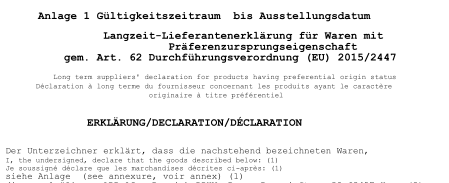
\includegraphics[width=1\textwidth]{img/Sprachen.png}}%		
		\caption{Mehrsprachige Lieferantenerklärung}
		\label{fig3}
	\end{figure}
	


	Die Zuweisung eines Formulars zu einer Gesellschaft findet im Customizing statt. Das Customizing ist ein separater Bereich im SAP, in welchem Einstellungen, Funktionen und Prozesse gesteuert werden. Im Fall der \ac{LLE} wird hier festgelegt, für welche Verwaltungseinheit welches Formular in der jeweiligen Verwaltungseinheit verwendet wird. In Abbildung \ref{fig4} ist zu sehen, dass bei Smart Forms zusätzlich auch noch ein Formulartext festgelegt werden kann, welcher im Formular verwendet werden kann.
	
		
	\begin{figure}[ht]
		\centering
		\makebox[\textwidth][c]{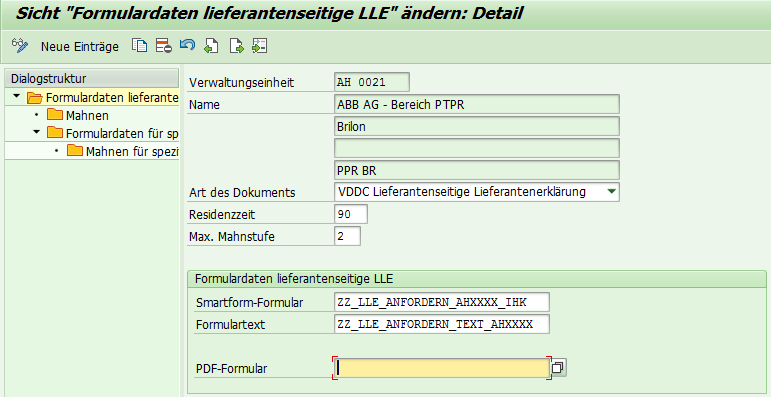
\includegraphics[width=1\textwidth]{img/Customizing.png}}	
		\caption{Customizing der Lieferantenerklärung }
		\label{fig4}
	\end{figure}

	Grundsätzlich funktioniert die \ac{LLE} in ihrem jetzigen Zustand, aber weitere Änderungen seitens der Zoll-Vorgaben oder der Gesellschaften führen immer mehr zu zusätzlichem Aufwand, welcher bei einer optimierten Lösung nicht nötig wäre. 

	\FloatBarrier
	
	\section{Schnittstelle in Smart Forms}
	
	Die Daten, welche zum Füllen der \ac{LLE} erforderlich sind, werden über eine Schnittstelle an das Formular übertragen. Diese Schnittstelle wird in Smart Forms definiert und besteht aus Import- und Export-Parametern, Tabellen und Ausnahmen. Die Import- beziehungsweise Export-Parameter beinhalten Definitionen, welche Daten dem Formular zur Verfügung stehen beziehungsweise Daten von dem Formular aus zurück an das Druckprogramm geben werden\footnote{Vgl. \cite{Hertleif.2003} S. 169 - 173}. Im Falle der \ac{LLE} beinhaltet die Schnittstelle neben den Standard-Parametern zwei Standard-SAP-Strukturen bei den Import-Parametern. Diese beinhalten alle Daten, welche für die \ac{LLE} relevant sind. Diese Strukturen müssen ebenfalls in der Schnittstelle des neuen Formulars vorhanden sein. Mit Hilfe der Ausnahmen in der Schnittstelle werden Fehler definiert, welche beim Auftreten keinen Programmabbruch herbeiführen sollen. Im Zusammenhang zur \ac{LLE} sind keine weiteren Ausnahmen definiert.    
	\section{Globale Definitionen}
	
	Nicht alle benötigten Daten für das Formular können über Standard-SAP-Strukturen in der Schnittstelle bereitgestellt werden. Hierfür können globale Definitionen erstellt werden, welche im gesamten Formular zur Verfügung stehen. Neben tatsächlichen Datenstrukturen ist es unter anderem möglich, Programmroutinen sowie Formroutinen für die Initialisierung des Dokumentes einzufügen\footnote{Vgl. \cite{Hertleif.2003} S. 176}. Für die \ac{LLE} sind diverse globale Daten definiert, welche im Formular an verschiedenen Stellen Anwendung finden. Ein großer Teil dieser Daten wird für das Auslesen von zusätzlichen Informationen aus dem SAP System benötigt. Definitionen, welche im neuen Formular unvermeidlich sind, müssen übernommen werden.
	
	
	\section{Inhalte der \acs{LLE}}
	
	Die Elemente in Smart Forms werden in einer Ordnerstruktur angezeigt. Im Folgenden wird diese Struktur analysiert und in gesellschaftsspezifische, harmonisier bare und einheitliche Inhalte unterteilt.
	Im Anhang \ref{AN:Smart1} sind die Elemente des Anschreibens von ABB aufgelistet. Jeder Punkt, welcher mit einem blauen Symbol versehen ist, ist mit einer Bedingung belegt, welche die Anzeige dieses Elements nur unter der Erfüllung selbiger zulässt. Somit ist sofort ersichtlich, dass der Punkt "`ANSCHREIBEN\_ANFORDERN\_TEXT"' keine Bedingung hat, das heißt, dieses Element wird für jede Gesellschaft gleich genutzt. Jedes andere Element findet nur unter bestimmten Bedingungen Verwendung. Das gesamte Anschreiben ist unterteilt in folgende Bereiche:
	
	\begin{itemize}
		\item Anschreiben
		\item Logos
		\item Adresskopf für Empfänger
		\item Adresskopf für die absendende Gesellschaft
		\item Adresskopf für den absendenden Mitarbeiter
		\item Fußzeile
		\item Sonstiges
	\end{itemize}

	Die Bedingungen prüfen fast ausschließlich die \ac{AH}-Nummern ab. Diese Nummer stellt im Falle der \ac{LLE} die Unterteilung der verschiedenen Gesellschaften dar.
\FloatBarrier


	\subsection{Anschreiben}
	
	Das Anschreiben ist für jede Gesellschaft gleich und trotzdem mit dynamischen Inhalten gefüllt. Das Jahr, ab welchem die \ac{LLE} gültig ist, steht mehrfach im Text. Zusätzlich stehen am Ende des Anschreibens der Firmenname sowie der Name des Ausstellers der \ac{LLE}. Diese Inhalte werden beim Drucken des Formulars eingesetzt.	
	
	\subsection{Logos}
	\label{ist_logos}
	
	Bei näherer Betrachtung der Logo-Elemente ist zu erkennen, dass die Grafiken in unterschiedlichen Weisen eingebunden werden. In Abbildung \ref{logo_smart} ist zu sehen, dass der Objektname, welcher auf die Grafik verweist\footnote{Grafiken können als "`GRAPHICS"' Objekt im SAP abgespeichert und über den definierten Namen an anderen Stellen eingefügt werden}, entweder fest eingetragen ist oder dynamisch eingefügt wird. 
	

	Es gibt insgesamt sechs Logo-Elemente, wobei zwei davon für eine Gesellschaft Anwendung finden. Die Elemente mit den Endungen "`BJ"', "`23XX"', "`KAUFEL"' und "`AT"' sind nur für bestimmte Gesellschaften, während das reine "`LOGO"'-Element für alle anderen Gesellschaften verwendet wird. Auffällig hierbei ist, dass für die \ac{AH} 3001, welche für die \ac{ABB} Österreich steht, zwei Logo-Elemente benötigt werden.
	Über die Positionierung ist zu erkennen, dass eines davon in der Fußzeile eingesetzt wird.
	
		\begin{figure}[ht]
		\centering
		\makebox[\textwidth][c]{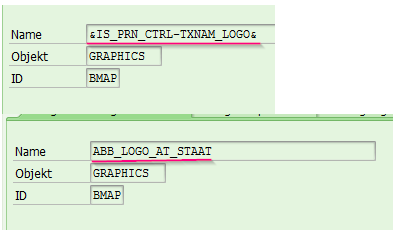
\includegraphics[width=9cm]{img/logo_smartform.png}}	
		\caption{Unterschiedliche Versionen der Logo-Einbindung in Smart Forms}
		\label{logo_smart}
	\end{figure} 
	Da aufgrund unterschiedlichen Brandings nicht für jede Gesellschaft dasselbe Logo verwendet werden kann, können die Logo-Elemente nicht harmonisiert werden.
	
	\subsection{Adressköpfe}
	\label{ist:adr}
	
	Das Anschreiben der \ac{LLE} beinhaltet drei verschiedene Adressköpfe. Einen für die Empfängeradresse, einen für die Adresse der Gesellschaft, welche die \ac{LLE} erstellt hat, sowie einen Adresskopf für den Mitarbeiter dieser Gesellschaft. Je nach Gesellschaft unterscheiden sich die Adressfelder im Inhalt beziehungsweise in der Position im Formular. Die Position kann hierbei vereinheitlicht werden, da sie sich im Smart Forms-Formular nur geringfügig unterscheidet und somit die Änderungen nicht sichtbar sein werden. 
	
	Teilweise können Adressen in Smart Forms als Textelemente dargestellt werden, welche über eine zugewiesene Adressnummer automatisch die zugehörigen Daten in einer definierbaren Struktur ausgeben. In Abbildung \ref{auto} ist die Definition eines solchen Feldes dargestellt. Die Adressnummer ist eine eindeutige Kennung für einen, im SAP System hinterlegten Adressdatensatz.
			\begin{figure}[ht]
			\centering
			\makebox[\textwidth][c]{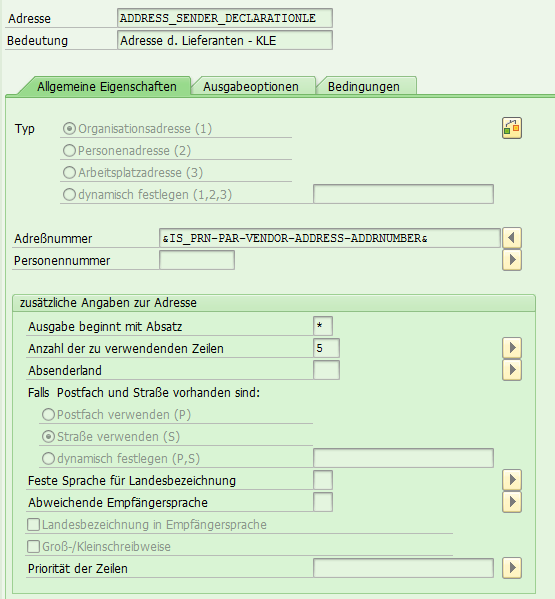
\includegraphics[width=9cm]{img/auto_adress.png}}	
			\caption{Automatischer Adresskopf in Smart Forms}
			\label{auto}
		\end{figure} 
	\FloatBarrier
	
	 Der Adressblock für die Empfängerdaten beinhaltet einen automatisch erstellten Adresskopf und Zusatzdaten in Form von einem Ansprechpartner sowie der Lieferantennummer. Über dem Adresskopf des Empfängers befindet sich die Absenderadresse in einer kleineren Version. Dieses Element ist für alle Gesellschaften gleich, außer für die \ac{AH} 2000, welche für die \ac{ABB} Tochtergesellschaft \ac{BJE} steht. Für diese Gesellschaft ist dieses Feld an der selben Stelle positioniert. Jedoch beinhaltet das Element nicht nur die Absenderadresse, sondern zusätzlich noch die Empfängerdaten, die für alle anderen Gesellschaften in dem bereits erwähnten separaten Element angelegt sind. Eine Möglichkeit der Harmonisierung ist somit gegeben, da es inhaltlich keine Unterschiede unter den Gesellschaften gibt.
	
	Die Kontaktdaten und Abteilungsdaten des Mitarbeiters, welcher die \ac{LLE} erstellt hat, werden auf dem Anschreiben oben rechts positioniert.
	Dem Smart Forms-Formular kann entnommen werden, dass es aktuell vier Elemente für diesen Adressblock gibt, welche im Anhang \ref{AN:Smart1} unter den Namen "`WINDOW\_USER\_AND-
	\_DEPARTMENT"' erkennbar sind. Für diese Daten wird kein Adressenelement verwendet, stattdessen ist ein Text definiert, der mit Variablen versehen ist. Mit Hilfe dieser Variablen wird der Text mit den benötigten Adressdaten gefüllt. Da bei näherer Betrachtung der Elementinhalte kein Unterschied feststellbar ist, können auch diese Inhalte zusammengeführt werden.
	
	Die Adresse der \ac{ABB}-Gesellschaft, welche die \ac{LLE} ausstellt, befindet sich über dem Adressblock des Mitarbeiters. Drei Elemente werden im Moment für dieses Feld eingesetzt. Das Element mit den Namen "`SENDER\_ADDRESS23XX"' ist auf dem Anschreiben weiter oben platziert als die beiden anderen Elemente und ist per Bedingung nur für die \ac{AH}s 0050, 0051 und 0053 gültig. Inhaltlich variieren die Elemente nicht, da sie alle gleich definierte Adressenfelder beinhalten. Auffällig ist, dass für die \ac{AH} 2000 keine Absenderadresse vorhanden ist. Dieser Umstand ist darauf zurückzuführen, dass sich das Logo dieser Gesellschaft an der Position befindet, an welcher sich das Adressfeld bei den anderen Gesellschaften befindet. Die drei Elemente können dementsprechend zu einem zusammengeführt werden, da es keinen Grund gibt, das Adressfeld an unterschiedlichen Positionen anzuzeigen. Für die \ac{BJE} darf dieses Adressfeld nicht angezeigt werden.
	
	\subsection{Sonstige Inhalte des Anschreibens}
	\label{ist:rueck}
	
	Für die \ac{AH}-Nummern 0050, 0051 und 0053 existiert noch ein weiteres Element mit dem Namen "`RUECK Neues Fenster 1"'. Dieses Feld beinhaltet eine Erinnerung an den Empfänger, dass dieses Dokument nur an die Abteilung des Absenders zurück geschickt werden darf. Um den gleichen Inhalt im neuen Formular beizubehalten, muss dieses Element auch im neuen Dokument vorhanden sein.
	
	Des Weiteren verwenden zwei Gesellschaften Fußzeilen, die ebenfalls in das neue Formular übertragen werden müssen. Eingebunden sind diese beiden Texte über Textbausteine.
	
	\subsection{Zweite Seite des Anschreibens}
	
	Im Anhang \ref{AN:Smart2} ist die Auflistung der Elemente auf der zweiten Seite des Anschreibens zu sehen. Es ist zu erkennen, dass alle Elemente dieser Seite denen der ersten Seite gleichen. Der einzige Unterschied hierbei ist der Zeitpunkt der Anzeige der einzelnen Elemente, welcher so eingestellt ist, dass diese nicht angezeigt werden. In Abbildung \ref{beding_smart} ist diese Bedingung dargestellt. Aufgrund dieser Einstellung ist die komplette zweite Seite nicht relevant für ein neues Formular und kann somit vernachlässigt werden. Zu einem früheren Zeitpunkt war die \ac{LLE} in einer anderen, größeren, Weise aufgebaut und das \ac{ABB}-Anschreiben benötigte aus dem Grund zwei Seiten.
	
	\begin{figure}[ht]
		\centering
		\makebox[\textwidth][c]{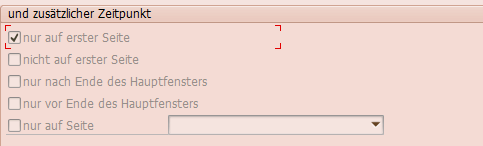
\includegraphics[width=9cm]{img/Anzeigebedingung_Smartform.png}}	
		\caption{Anzeigezeitpunkt der zweiten Seite in Smart Forms}
		\label{beding_smart}
	\end{figure}
	
	\subsection{Anschreiben der \acs{LLE}}
	\label{ist:le}
	
	Zusätzlich zum Anschreiben der \ac{ABB} gibt es noch ein Anschreiben, welches inhaltlich vom Zoll vorgegeben ist. Dieser Text beschreibt die Bedeutung des Dokumentes und bildet die tatsächliche "`Erklärung"' in der \ac{LLE}. Der Unterordner "`PREF Formulare 1"' im Anhang \ref{AN:Smart3} beinhaltet die Elemente dieser Seite. Zum einen beinhaltet der Ordner den vorgegebenen Zolltext und eine Logik für die Seitenzahlen und zum anderen ein Element, welches dynamische Inhalte des Textes füllt. Zu diesen dynamischen Inhalten gehören Angaben zum Datum, sowie Adress- beziehungsweise Kontaktdaten. Der Knoten "`DATEN ERMITTELN"' beinhaltet ein selbstgeschriebenes Programm, welches die Daten für den folgenden Teil der \ac{LLE} aufbereitet. Da die komplette Seite unabhängig von den Gesellschaften ist, bietet sich die Möglichkeit, diese in das neue Formular zu übernehmen. 
	
	\subsection{Materialliste}
	
	Ein Teil der \ac{LLE} bildet eine Auflistung von Materialien. Diese Liste kann beliebig lang sein und besteht aus sieben Spalten. Im Anhang \ref{AN:Smart3} ist zu sehen, dass die Seite dieser Liste aus fünf Elementen besteht: einer Logik für die Seitenzahlen, Aussteller- und Empfänger-Daten der \ac{LLE}, Adressdaten von Absender und Adressat und einem Element für die Liste selbst.
	In Abbildung \ref{list_smart} ist der Aufbau des Listen-Elements dargestellt.
	
	\begin{figure}[ht]
		\centering
		\makebox[\textwidth][c]{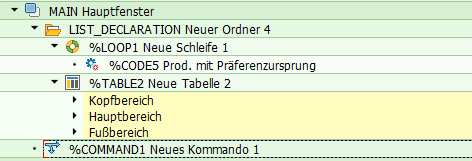
\includegraphics[width=9cm]{img/Liste_Smartform.png}}	
		\caption{Aufbau des Listen-Elements in Smart Forms}
		\label{list_smart}
	\end{figure}
	
	Eine Schleife wird dafür genutzt, jede Zeile der Liste mit Inhalt zu füllen. Abschließend wird ein Kommandoelement für die Weiterleitung auf die nächste Seite benötigt, da beliebig viele Seiten mit dieser Liste gefüllt werden können.
	
	Die einzige Bedingung, mit welcher die Elemente dieser Seite verknüpft sind, ist, dass ein präferenzberechtigtes Material\footnote{Siehe Kapitel \ref{LLE}} vorliegen muss. Da diese Bedingung für alle Gesellschaften gilt und sonst keine weiteren Bedingungen oder sonstige Unterschiede festzustellen sind, kann diese Seite ebenfalls in das neue Formular übernommen werden. 
	
	\subsection{Legende}
	\label{ist:leg}
	
	Die Seite nach der Materialliste besteht aus einer Legende, welche Abkürzungen von Abkommen, die in der Materialliste verwendet werden, auflistet. Diese Liste ist immer identisch und kann somit direkt im neuen Formular eingesetzt werden.
	
	
	\subsection{Sonstige Seiten}
	
	Im Anhang \ref{AN:Smart3} sind weitere Seiten aufgelistet, welche obsolete Inhalte vorhergegangener Versionen der \ac{LLE} sind. Diese Seiten werden aktuell durch Anzeigezeitpunkte ausgeblendet. Sie wurden bisher nicht gelöscht, um eventuelle Wiedereinführungen einfacher zu gestalten.
	Das neue Formular wird nach den aktuellen Vorgaben\footnote{Vgl. \cite{ZOLL.2017}} des Zolls aufgebaut sein und somit diese Seiten nicht weiter beinhalten.
	
	
	\FloatBarrier
	\section{Anforderungen}
	\label{ch:Anf}
		Die Grundanforderung an das neue Formular ist, dass zum Ende der Arbeit inhaltlich das identische Dokument - auf Basis der Interactive Forms - ausgedruckt wird, wie mit Smart Forms. Optisch soll kein Unterschied für die operativen Einheiten zu erkennen sein. Darüber hinaus ist es sehr wichtig, dass die Fachbereiche nicht durch Einarbeitungszeit oder längere Umstellungsprozesse beeinträchtigt werden. 
	
		Gesellschaftsspezifische Inhalte, wie beispielsweise Logos, sollen weiterhin dynamisch angedruckt werden.
		Die Adressfelder, welche in dem Smart Forms-Formular unterschiedlich sind, werden vereinheitlicht, um das Dokument technisch gesehen übersichtlicher zu gestalten. Trotz der Harmonisierung sollen weiterhin alle Daten angezeigt werden, die aktuell auf dem Formular stehen. 
		
		Um zukünftige Änderungen am Formular zu vereinfachen, müssen alle Elemente und Komponenten des Adobe \ac{PDF}s kongruent und leicht verständlich benannt sein. Wird bei der Erstellung des Formulars kein System verfolgt, kann es dazu führen, dass erneut ein erhöhter Einarbeitungsaufwand erforderlich wird. In der Vergangenheit bestand die \ac{LLE} aus zwei Teilen welche dann zusammengeführt wurden. Solche Änderungen sind auch in der Zukunft zu erwarten. Außerdem können Änderungen im Branding einer Gesellschaft zu hohen Arbeitsaufwänden führen, solange das Formular weiterhin in einem so komplexen Zustand verwendet wird. Änderungen seitens der Texte innerhalb der \ac{LLE} sind ebenfalls möglich. Ein Beispiel ist hierfür das neue Freihandelsabkommen mit Kanada, welches seit neustem Teil der Legende ist\footnote{Vgl. \cite{ZOLL.2017b}}.
		
		Für die \ac{LLE} ist es nicht von Nöten, eine optimierte Art der automatischen Übersetzung der Texte zu finden, da alle nötigen Sprachen (Deutsch, Englisch und Französisch) gleichzeitig im selben Formular aufgedruckt werden. Eine Übersetzung wäre jedoch durch die Standard-SAP-Funktion möglich, ist aber nicht gewünscht beziehungsweise erforderlich.
		
